\documentclass{beamer}

\usepackage{lmodern}

\usepackage{listings}


\usepackage{algorithm}
\usepackage{algpseudocode}
\usepackage{amsmath}

\usepackage[T2A]{fontenc}
\usepackage[utf8]{inputenc}

\usetheme{Madrid}
\usecolortheme{beaver}

\title[]{Размещение реплик в распределенной\\системе на базе Erlang-процессов}
\author[Быцюк В.В.]{Быцюк Владислав Вячеславович}
\date[]{}

\begin{document}
	\setbeamertemplate{caption}{\raggedright\insertcaption\par}

% Титульный лист
\begin{frame}
	\titlepage
	\begin{center}
		Научный руководитель:\\д.ф.-м.н., профессор В.С. Пилиди\\~\\

		Рецензент:\\к.ф.-м.н., доцент С.А. Гуда\\~\\

		Прикладная математика и информатика

		Кафедра информатики и вычислительного эксперимента
	\end{center}
\end{frame}

% Постановка задачи
\begin{frame}{\LARGE \textbf{Постановка задачи}}
	\begin{itemize}
		\item Реализовать распределенное клиент-серверное приложение для хранения данных на языке программирования Erlang. 
    	\item Реализовать алгоритм размещения реплик объектов в распределенной сети. 
    	\item Провести замеры количества итераций алгоритма и проанализировать полученные результаты.
	\end{itemize}
\end{frame}
	
	
% Основное содержание

\begin{frame}[fragile]{Erlang-процессы}
	\begin{block}{Запуск процесса}
		\begin{lstlisting}[language = erlang] 	
Pid = spawn(Fun).
		\end{lstlisting}
	\end{block}	

	\begin{block}{Отправка сообщения}
		\begin{lstlisting}[language = erlang] 	
Pid ! Message.
		\end{lstlisting}
	\end{block}	

	\begin{block}{Ожидание сообщений}
		\begin{lstlisting}[language = erlang] 	
receive
  Pattern1 -> Expressions1;
  Pattern2 -> Expressions2;
  true     -> Expression3
end
		\end{lstlisting}
	\end{block}	
\end{frame}

\begin{frame}[fragile]{Клиент-серверное приложение}
	\begin{figure}
		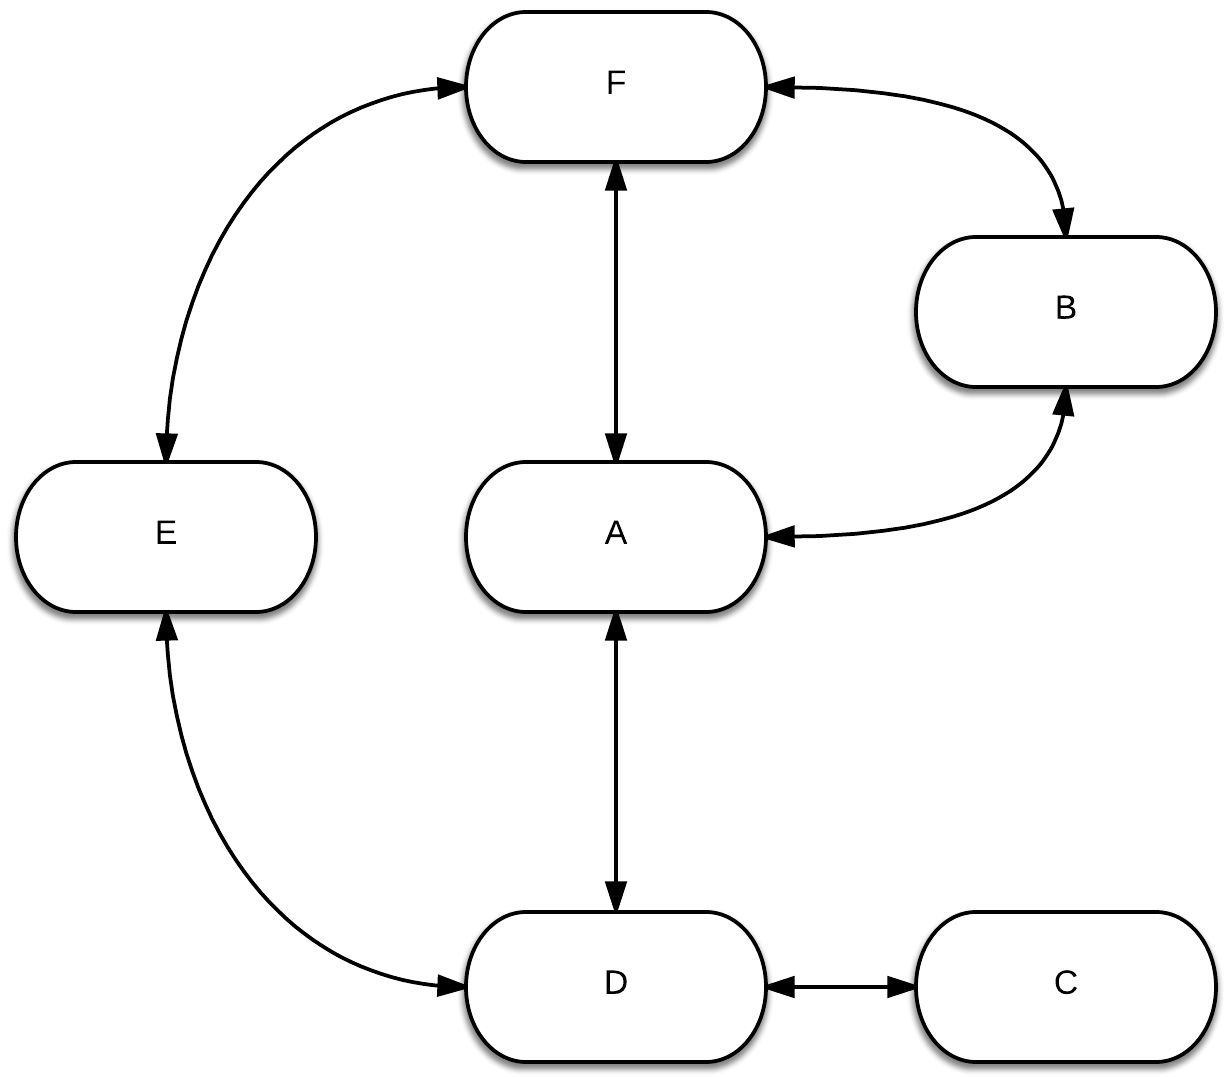
\includegraphics[scale=0.18]{img/example.png}
		\caption{Пример произвольной топологии системы}
	\end{figure}
\end{frame}
	
\begin{frame}[fragile]{Клиент-серверное приложение}
	\begin{figure}
		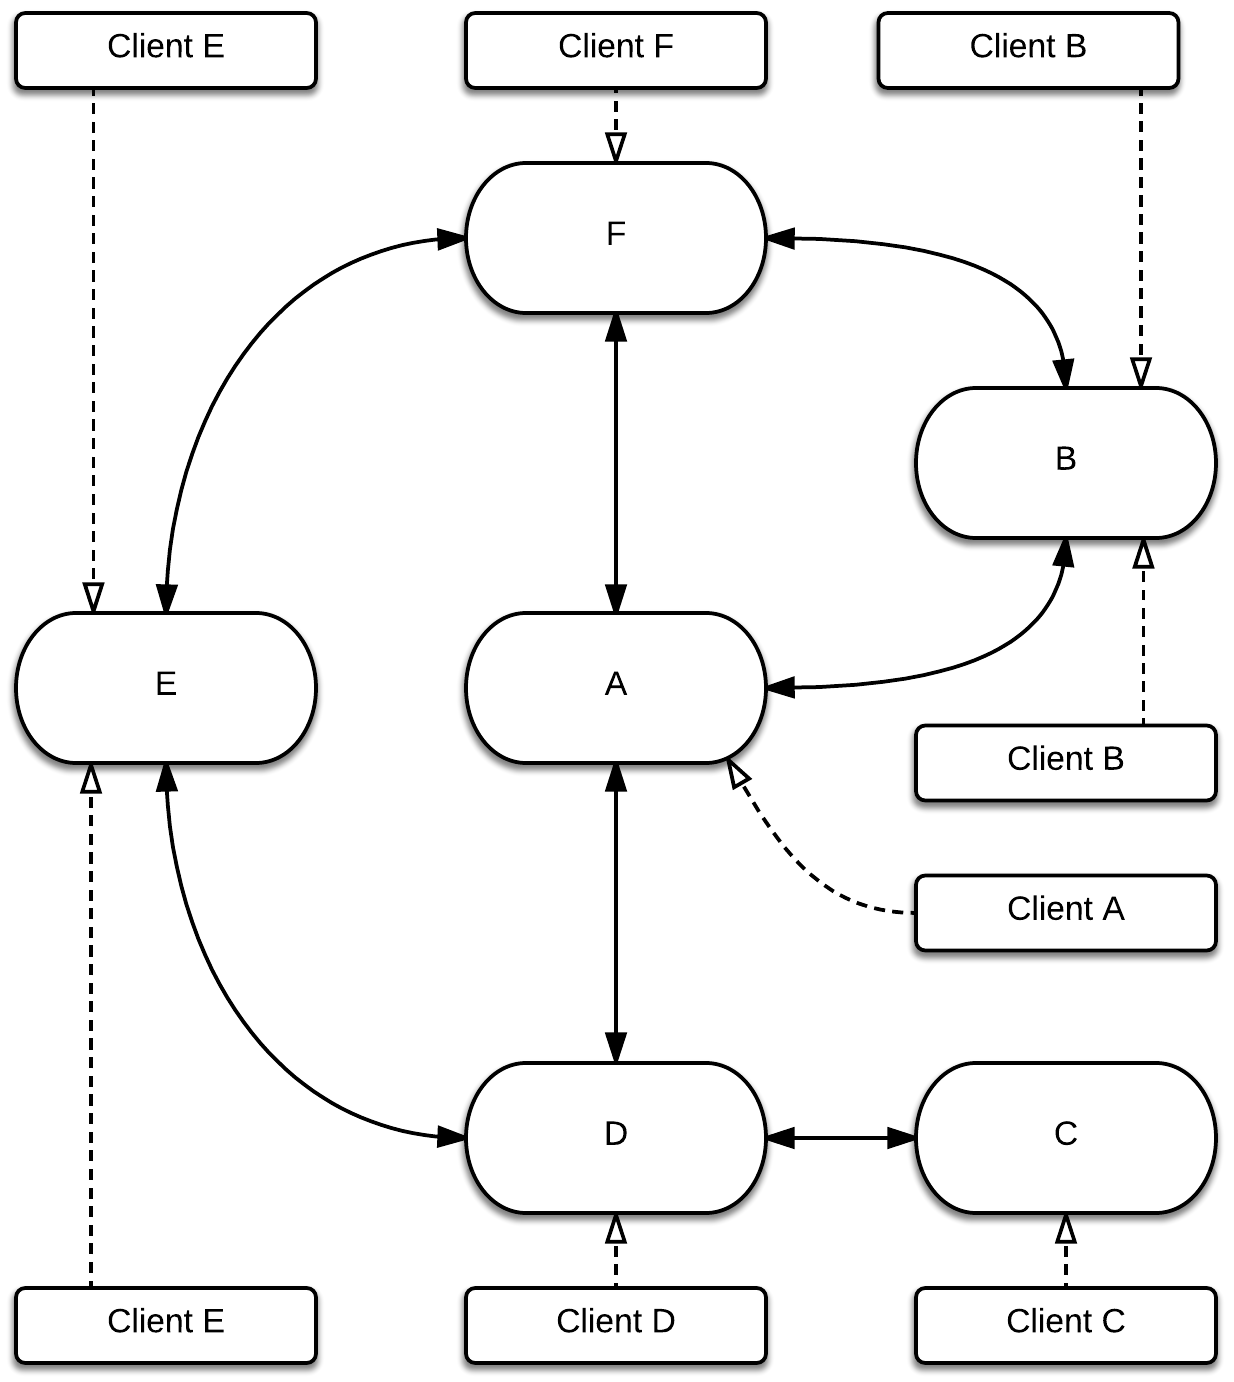
\includegraphics[scale=0.14]{img/client_ex.png}
		\caption{Пример системы с клиентами}
	\end{figure}
\end{frame}

\begin{frame}[fragile]{Клиент-серверное приложение}
	\begin{figure}
		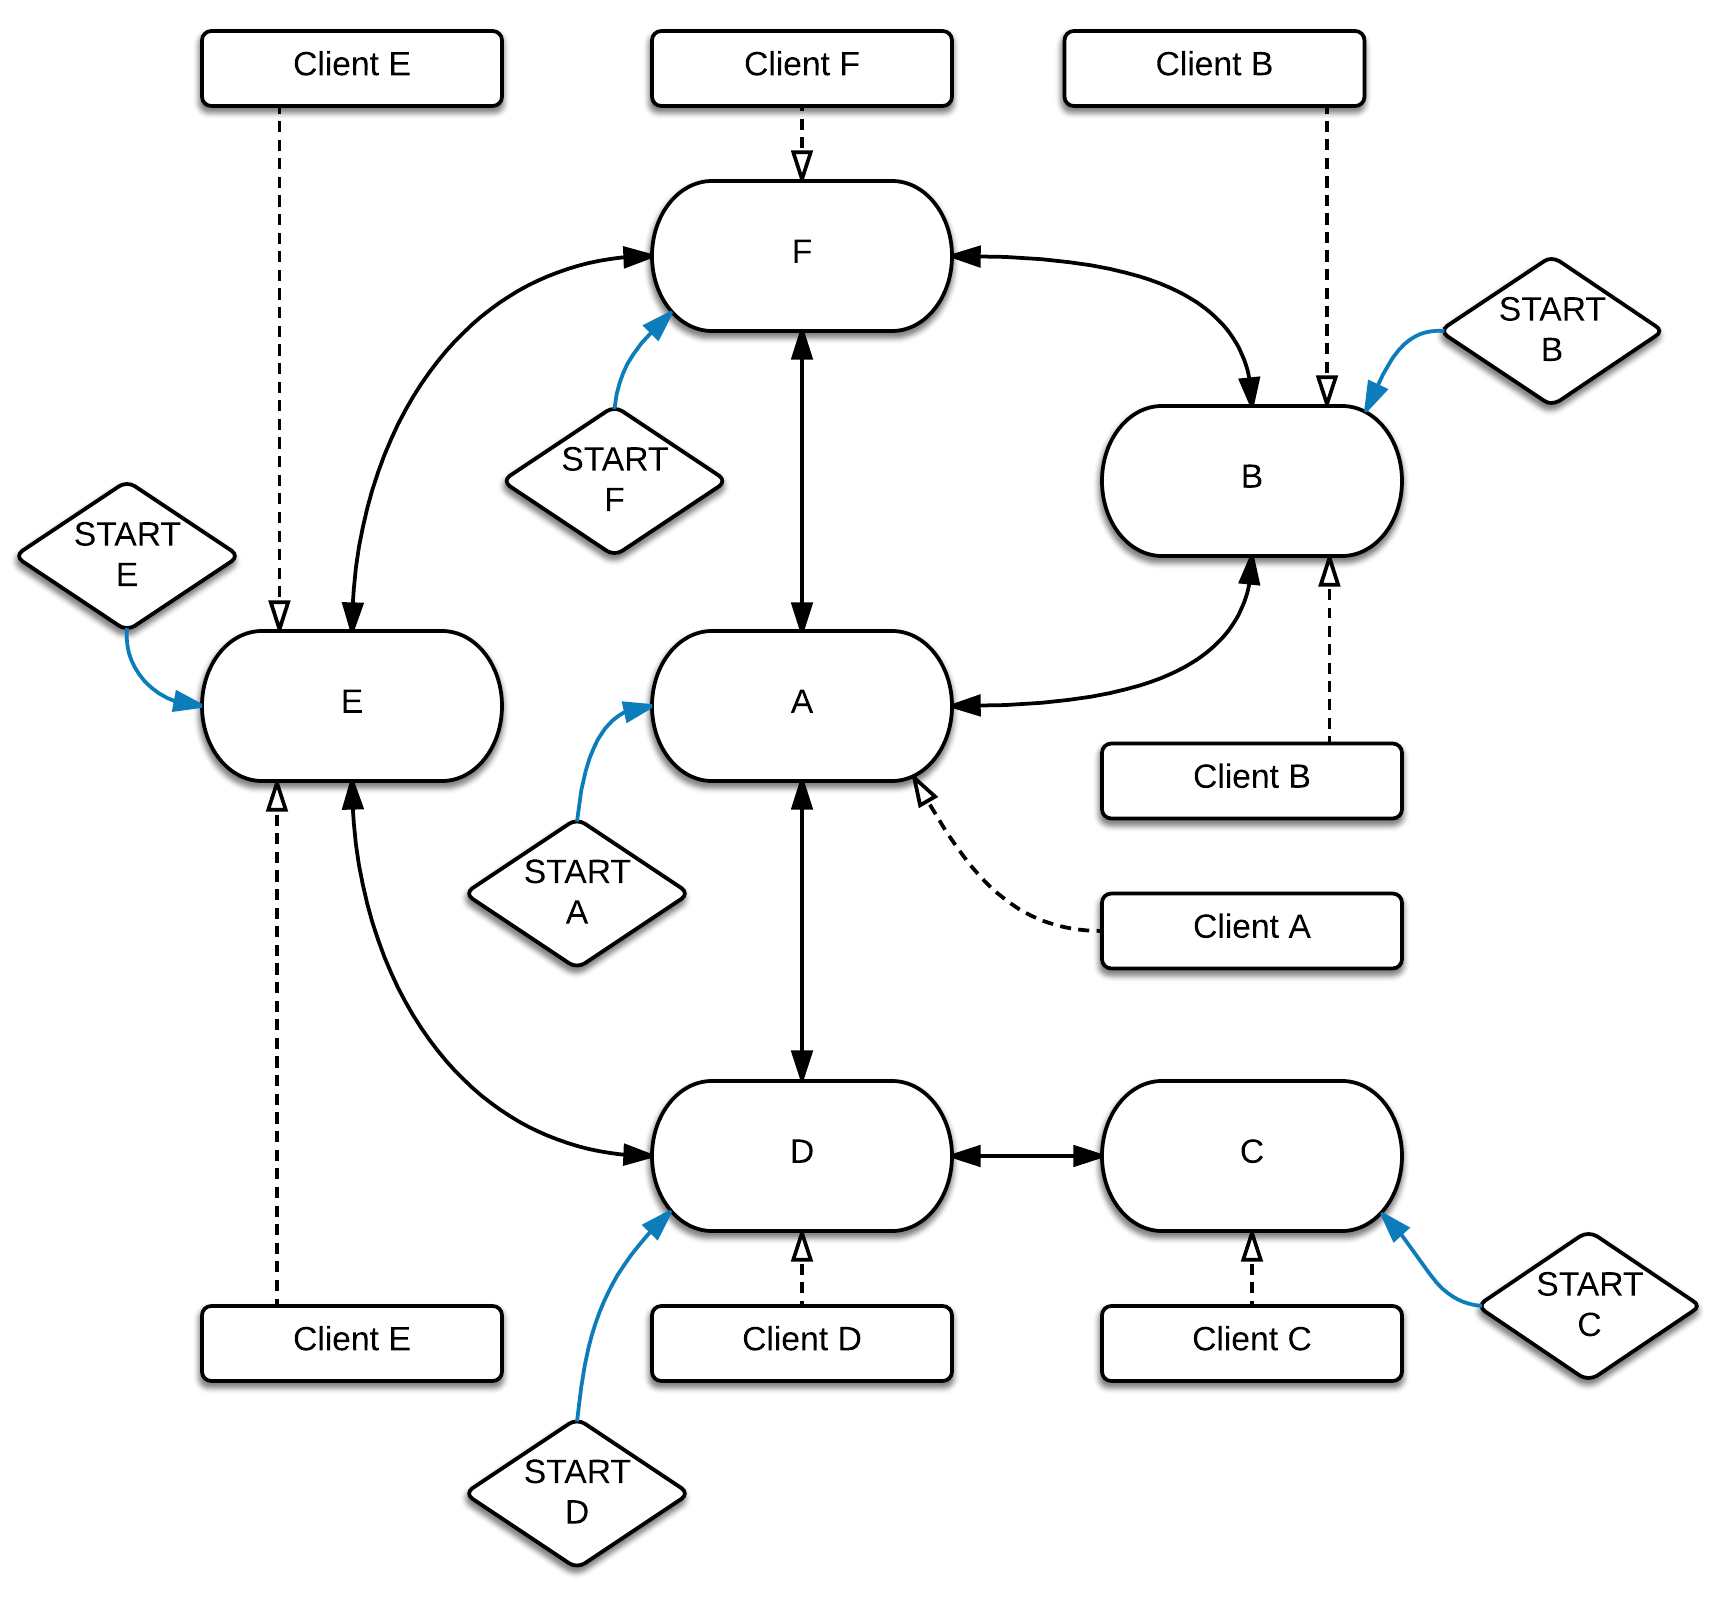
\includegraphics[scale=0.11]{img/start.png}
		\caption{Пример системы с клиентами и процессами запуска}
	\end{figure}
\end{frame}

\begin{frame}[fragile]{Клиент-серверное приложение}
	\begin{figure}
		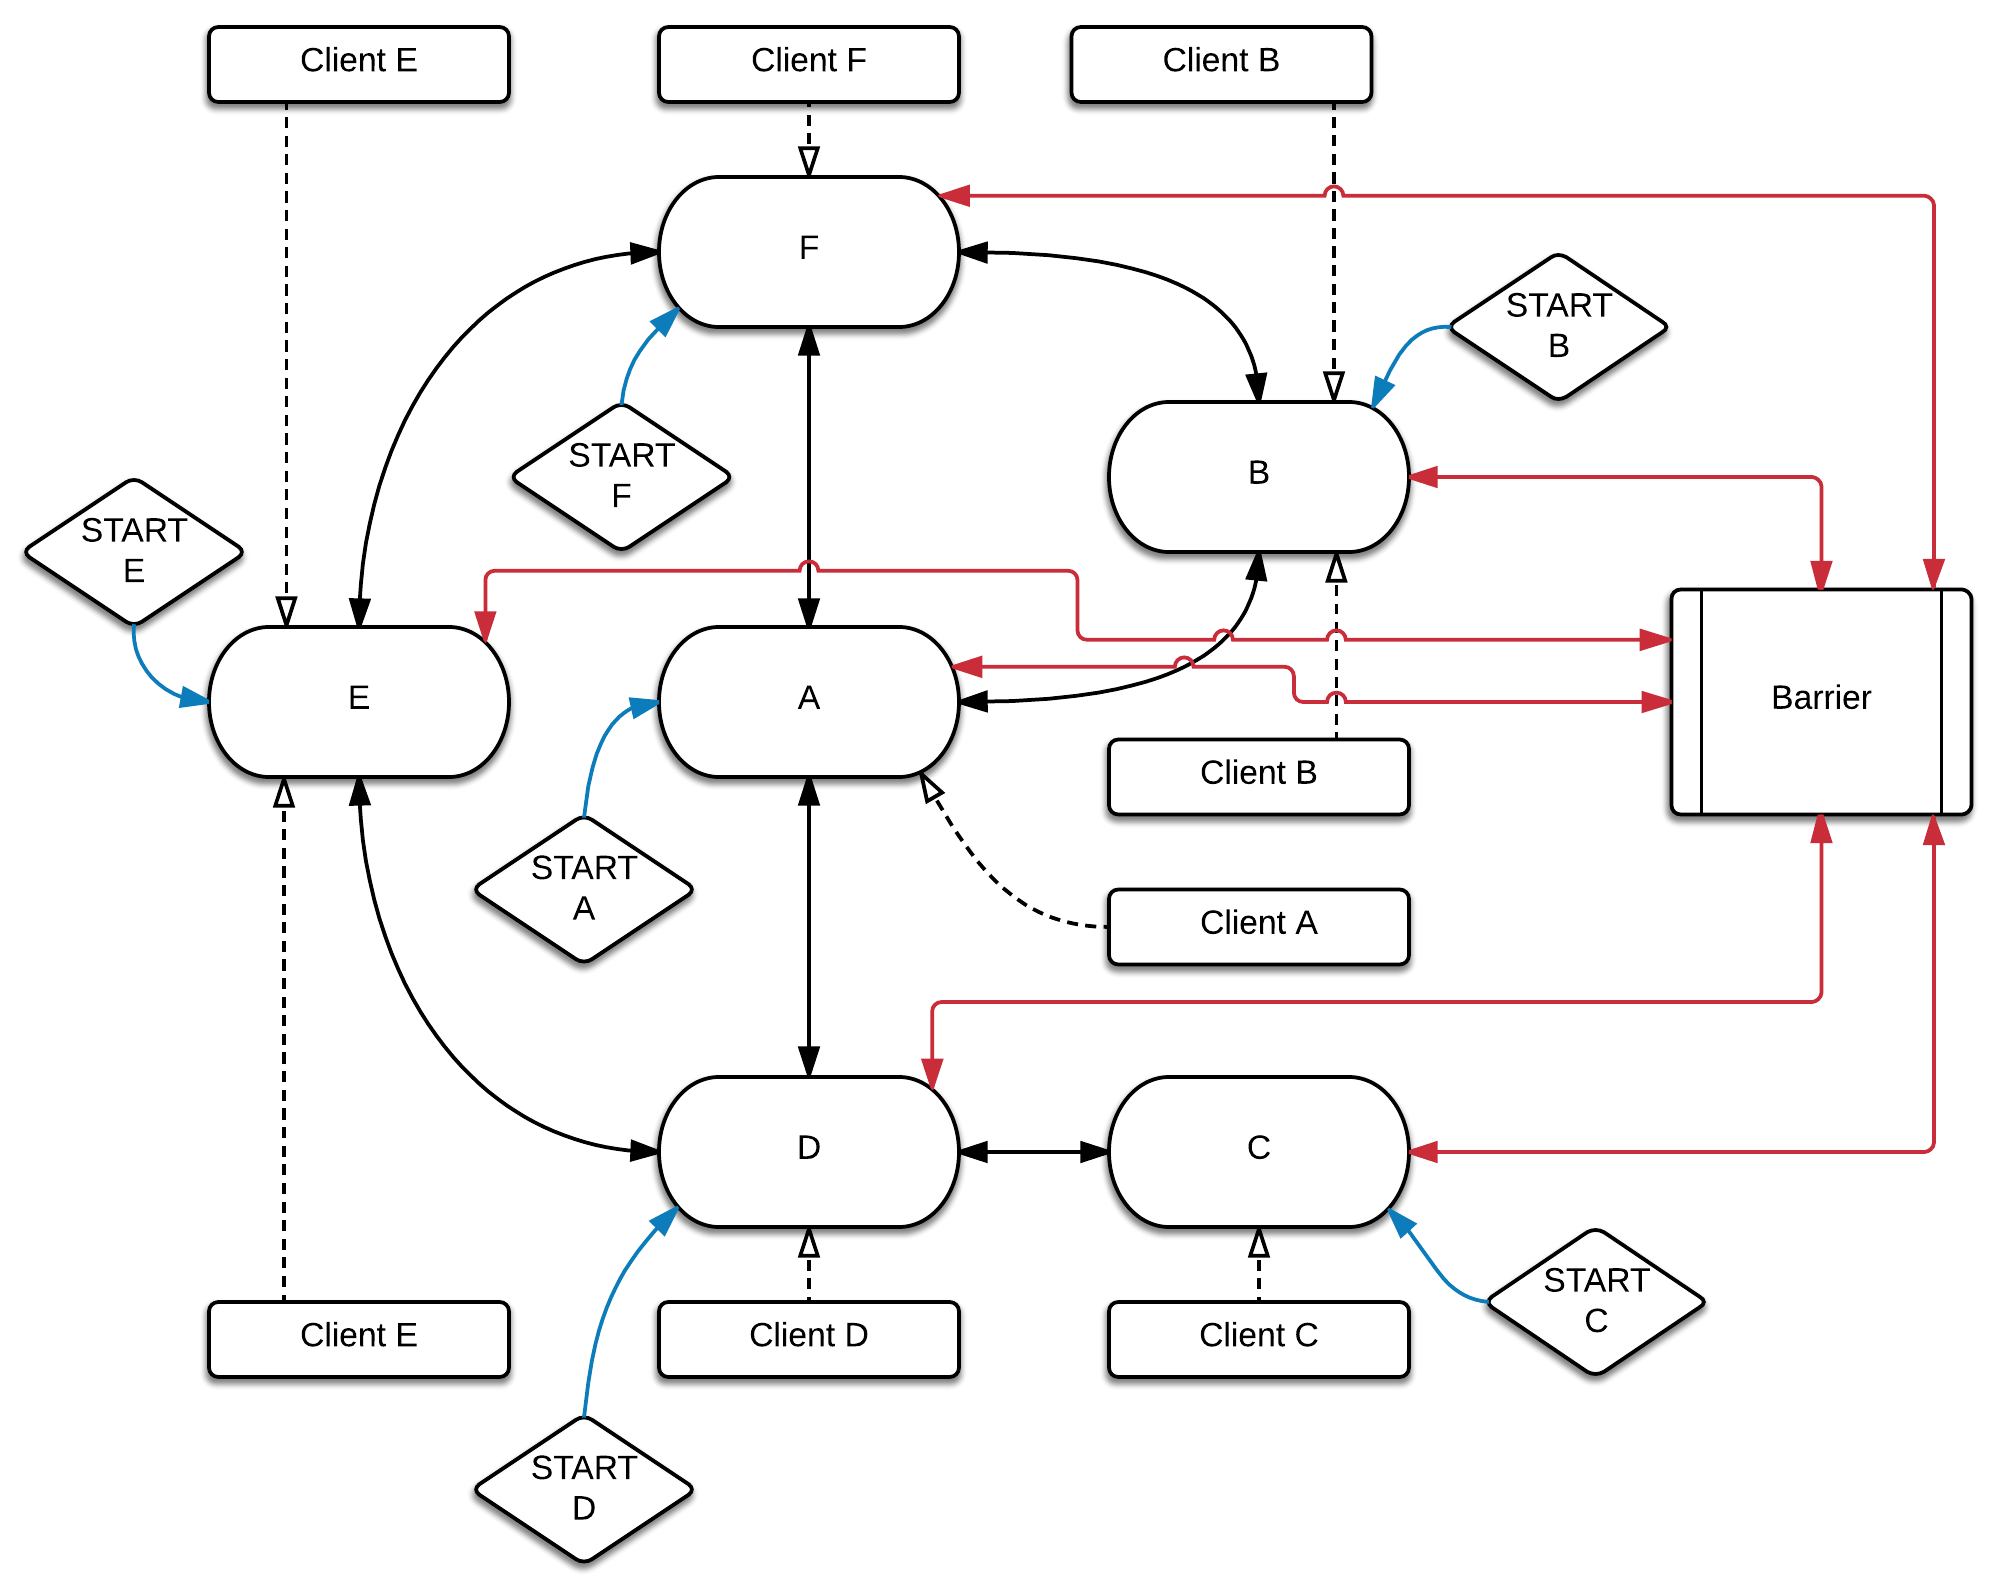
\includegraphics[scale=0.11]{img/bar.png}
		\caption{Пример системы с клиентами, процессами запуска и процессом барьера}
	\end{figure}
\end{frame}

\begin{frame}[fragile]{Основные обозначения}
	$s_1, \ldots, s_m$~---~сервера,\quad$o_1, \ldots, o_n$~---~объекты,\quad$c_1, \ldots, c_m$~---~емкости~серверов\\~\\
	
	$t_l$ --- время доступа к объекту хранящемуся на текущем сервере\\
	$t_r$ --- время доступа к объекту хранящемуся на соседнем сервере\\
	$t_s$ --- время доступа к объекту хранящемуся на удаленном сервере\\~\\

	$rc_j$ --- количество копий объекта $o_j$ на всех серверах\\
	$r_{ij}$ --- количество запросов к объекту $o_j$ с сервера $s_i$\\
	$p_j = \sum_{i=1}^{m} r_{ij}$ --- количество запросов к объекту $o_j$ со всех серверов\\~\\
\end{frame}

\begin{frame}[fragile]{Основные обозначения}
	$X_{ij}$ --- флаг, говорящий о том, размещен ли объект $o_j$ на сервере $s_i$
	\[ 	
		X_{ij} =
		\begin{cases} 
			1 & o_j \in s_i \\ 
			0 & o_j \notin s_i 
		\end{cases}
	\] 
	$ig_{ij}$ --- выгода от вставки объекта $o_j$ на сервер $s_i$
	\[ 	
		ig_{ij} =
		\begin{cases} 
			p_j (t_s - t_r) + r_{ij} (t_r - t_l) 	& rc_j = 0 \\
			r_{ij} (t_r - t_l) 						& X_{ij} = 0, rc_j > 0 \\
			0 										& X_{ij} = 1 
		\end{cases}
	\] 
	$ec_{ij}$ --- стоимость удаления объекта $o_j$ с сервера $s_i$
	\[ 	
		ec_{ij} =
		\begin{cases} 
			0										& X_{ij} = 0 \\
			r_{ij} (t_r - t_l) 						& X_{ij} = 1, rc_j > 0 \\
			p_j (t_s - t_r) + r_{ij} (t_r - t_l)	& X_{ij} = 1, rc_j = 1 
		\end{cases}
	\] 
\end{frame}

\begin{frame}[fragile]{Алгоритм}
	\begin{block}{Шаг 1. Инициализация.}
		\textbf{all-reduce-sum}($r_i, p$)\\
		$X_i \gets 0$\\
		$e_i \gets c_i$\\
		$for$ $j$ $:=$ $1$ $to$ $n$ $do$\\
		\qquad$ig_{ij} \gets p_j (t_s - t_r) + r_{ij} (t_r - t_l)$\\
		\qquad$ec_{ij} \gets 0$\\
		\qquad$rc_j \gets 0$
	\end{block}

	\begin{block}{Шаг 2. Выбор элемента с максимальной выгодой вставки.}
		$ig_{max} \gets max_k (ig_{ik})$\\
		$j \gets arg(max_k(ig_{ik})$\\
		$send\_msg \gets (ig_{max}, i, j, 0)$\\ 
		\textbf{all-reduce-max}($send\_msg, recv\_msg$)\\
		$(ig_{max}, i', j, j') \gets recv\_msg$		
	\end{block} 
\end{frame}

\begin{frame}[fragile]{Алгоритм}
	\begin{block}{Шаг 3. Условие остановки.}
		$if$ $ig_{max} \le 0$ $then$ $stop$
	\end{block}

	\begin{block}{Шаг 4.1. Если $i = i'$}
		$X_{ij} \gets 1$\\
		$ec_{ij} \gets ig_{ij}$\\
		$ig_{ij} \gets 0$\\
		$e_i \gets e_i - 1$\\
		$rc_j \gets rc_j + 1$\\
		$if$ $j' \neq 0$ $then$\\
		\qquad$X_{ij'} \gets 0$\\
		\qquad$ig_{ij'} \gets ec_{ij'}$\\
		\qquad$ec_{ij'} \gets 0$\\
		\qquad$e_i \gets e_i + 1$\\
		\qquad$rc_{j'} \gets rc_{j'} - 1$
	\end{block}
\end{frame}

\begin{frame}[fragile]{Алгоритм}
	\begin{block}{Шаг 4.2. Если $i \ne i'$}
		$rc_j \gets rc_j + 1$\\
		$if$ $X_{ij} = 0$ $then$\\
		\qquad$ig_{ij} \gets r_{ij} (t_r - t_l)$\\
		$else$\\
		\qquad$ec_{ij} \gets r_{ij} (t_r - t_l)$\\
		$if$ $j' \neq 0$ $then$\\
		\qquad$rc_{j'} \gets rc_{j'} - 1$\\
		\qquad$if$ $X_{ij'} = 1$ and $rc_{j'} = 1$ $then$\\
		\qquad\qquad$ec_{ij'} \gets r_{ij'} (t_r - t_l) + p_{j'} (t_s - t_r)$
	\end{block}
\end{frame}

\begin{frame}[fragile]{Алгоритм}
	\begin{block}{Шаг 5. Подготовка к следующей итерации.}
		$ig_{max} \gets max_k (ig_{ik})$\\
		$j \gets arg(max_k(ig_{ik})$\\
		$ec_{min} \gets min_k (ec_{ik} : ec_{ik} > 0)$\\
		$j' \gets arg(min_k(ec_{ik} : ec_{ik} > 0)$\\
		$if$ $e_i = 0$ or $c_i - e_i \ge n$ $then$\\
		\qquad$if$ $ig_{max} \le ec_{min}$ $then$\\
		\qquad\qquad$ig_{max} \gets 0$\\
		\qquad\qquad$j' \gets 0$\\
		$else$\\ 
		\qquad$j' \gets 0$\\
	\end{block}
\end{frame}

\begin{frame}[fragile]{Алгоритм}	
	\begin{block}{Шаг 6. Выбор элемента с максималной выгодой вставки.}
		$send\_msg \gets (ig_{max}, i, j, j')$\\
		\textbf{all-reduce-max}($send\_msg, recv\_msg$)\\
		$(ig_{max}, i', j, j') \gets recv\_msg$\\
		$goto$ $3$
	\end{block}
\end{frame}


\begin{frame}[fragile]{Тестовые испытания}
	\begin{figure}
		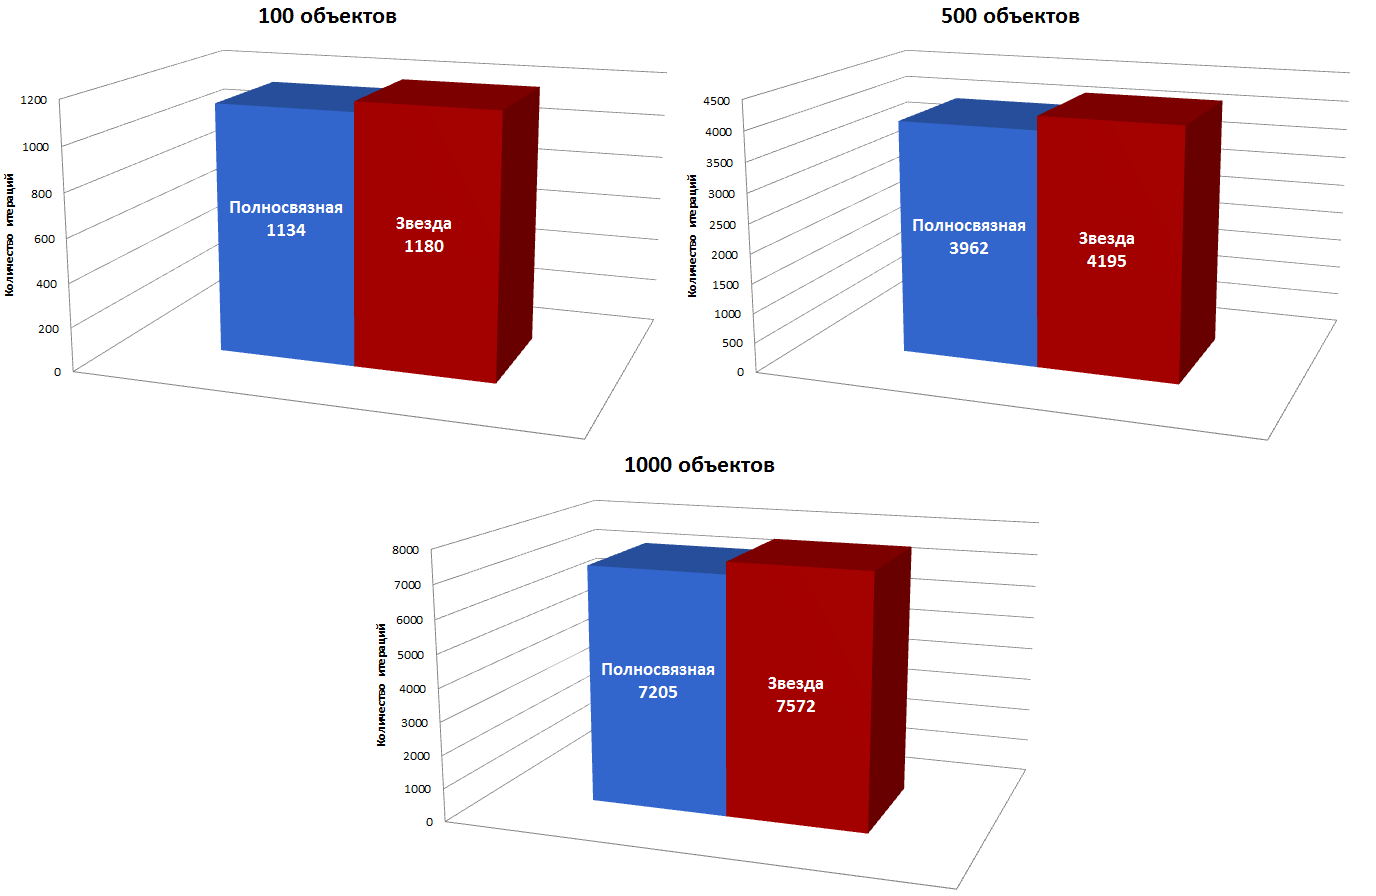
\includegraphics[scale=0.2]{img/histograms/top.png}
		\caption{Влияние топологии сети на количество итераций алгоритма}
	\end{figure}
\end{frame}

\begin{frame}[fragile]{Тестовые испытания}
	\begin{figure}
		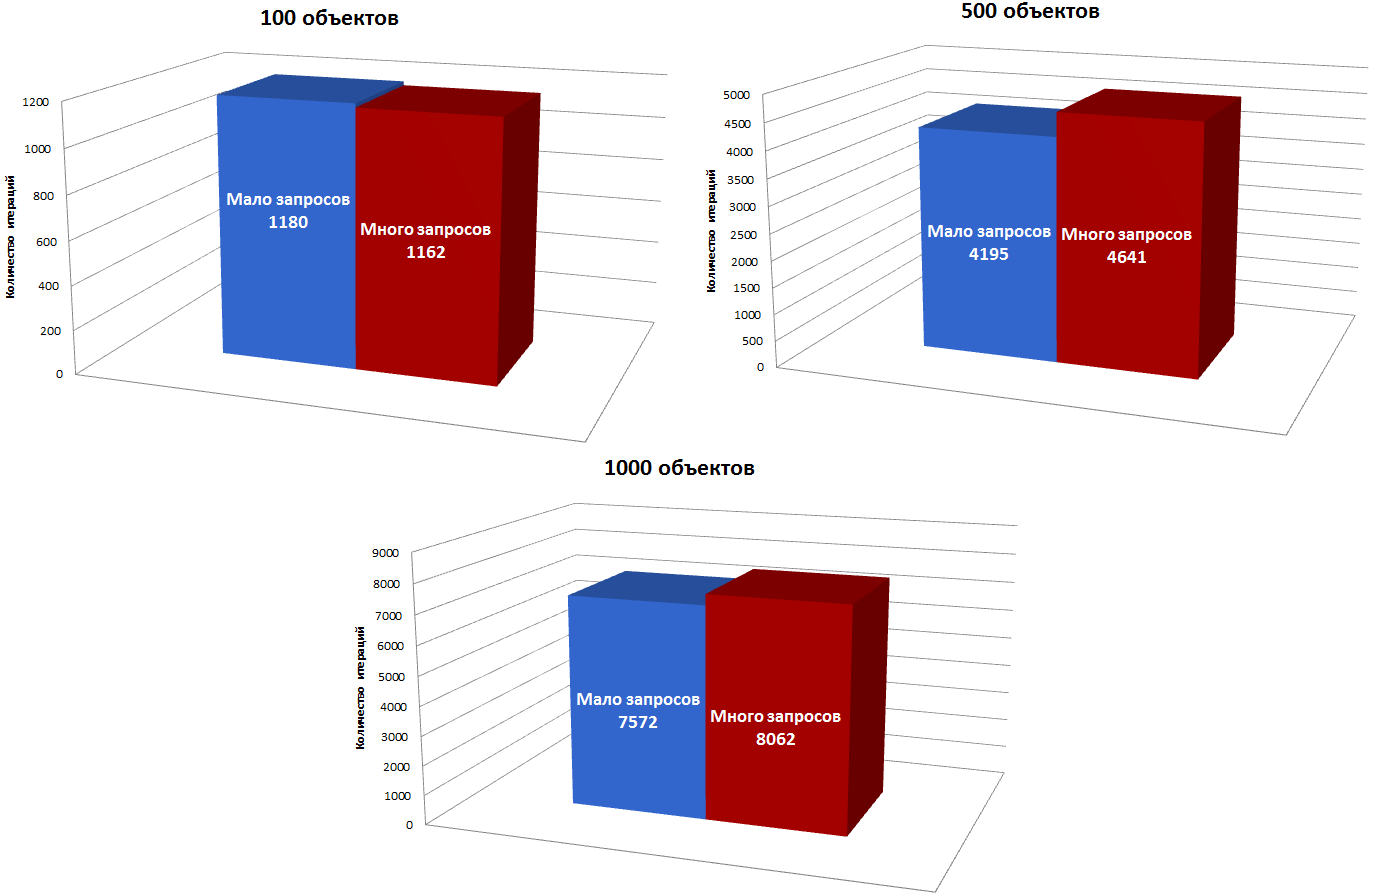
\includegraphics[scale=0.2]{img/histograms/req.png}
		\caption{Влияние общего количества запросов к объекту на количество итераций алгоритма}
	\end{figure}
\end{frame}

\begin{frame}[fragile]{Тестовые испытания}
	\begin{figure}
		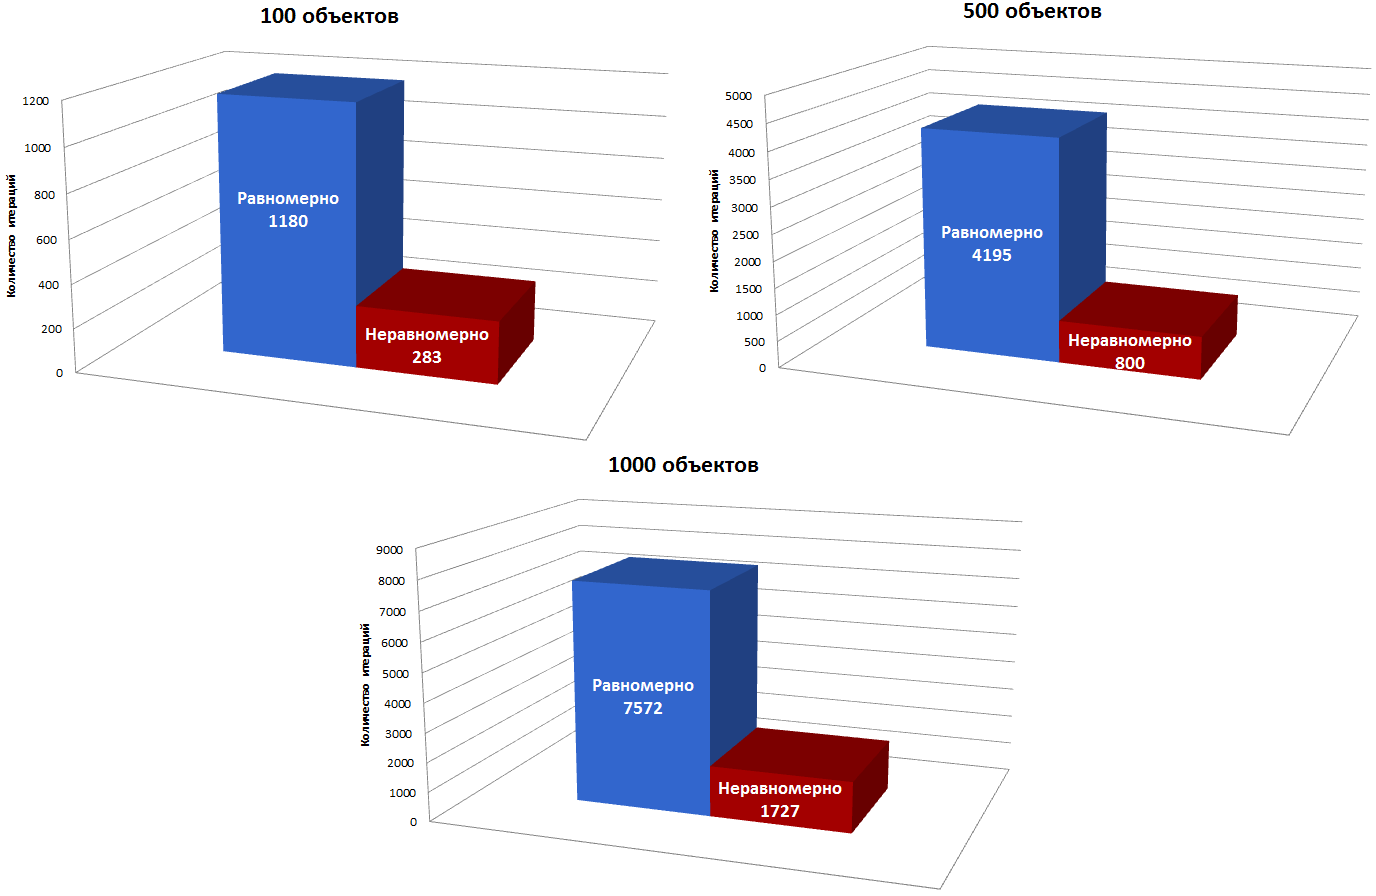
\includegraphics[scale=0.2]{img/histograms/dist.png}
		\caption{Влияние распределения запросов к объектам на количество итераций алгоритма}
	\end{figure}
\end{frame}


% Полученные результаты
\begin{frame}{Полученные результаты}
	\begin{itemize}
		\item Реализовано распределенное клиент-серверное приложение для хранения данных на языке программирования Erlang. 
    	\item Реализован алгоритм размещения реплик объектов в распределенной сети. 
    	\item Проведены замеры количества итераций алгоритма и проанализированы полученные результаты.
	\end{itemize}
\end{frame}

\end{document}
